% Created by tikzDevice version 0.12.3 on 2021-01-17 19:46:18
% !TEX encoding = UTF-8 Unicode
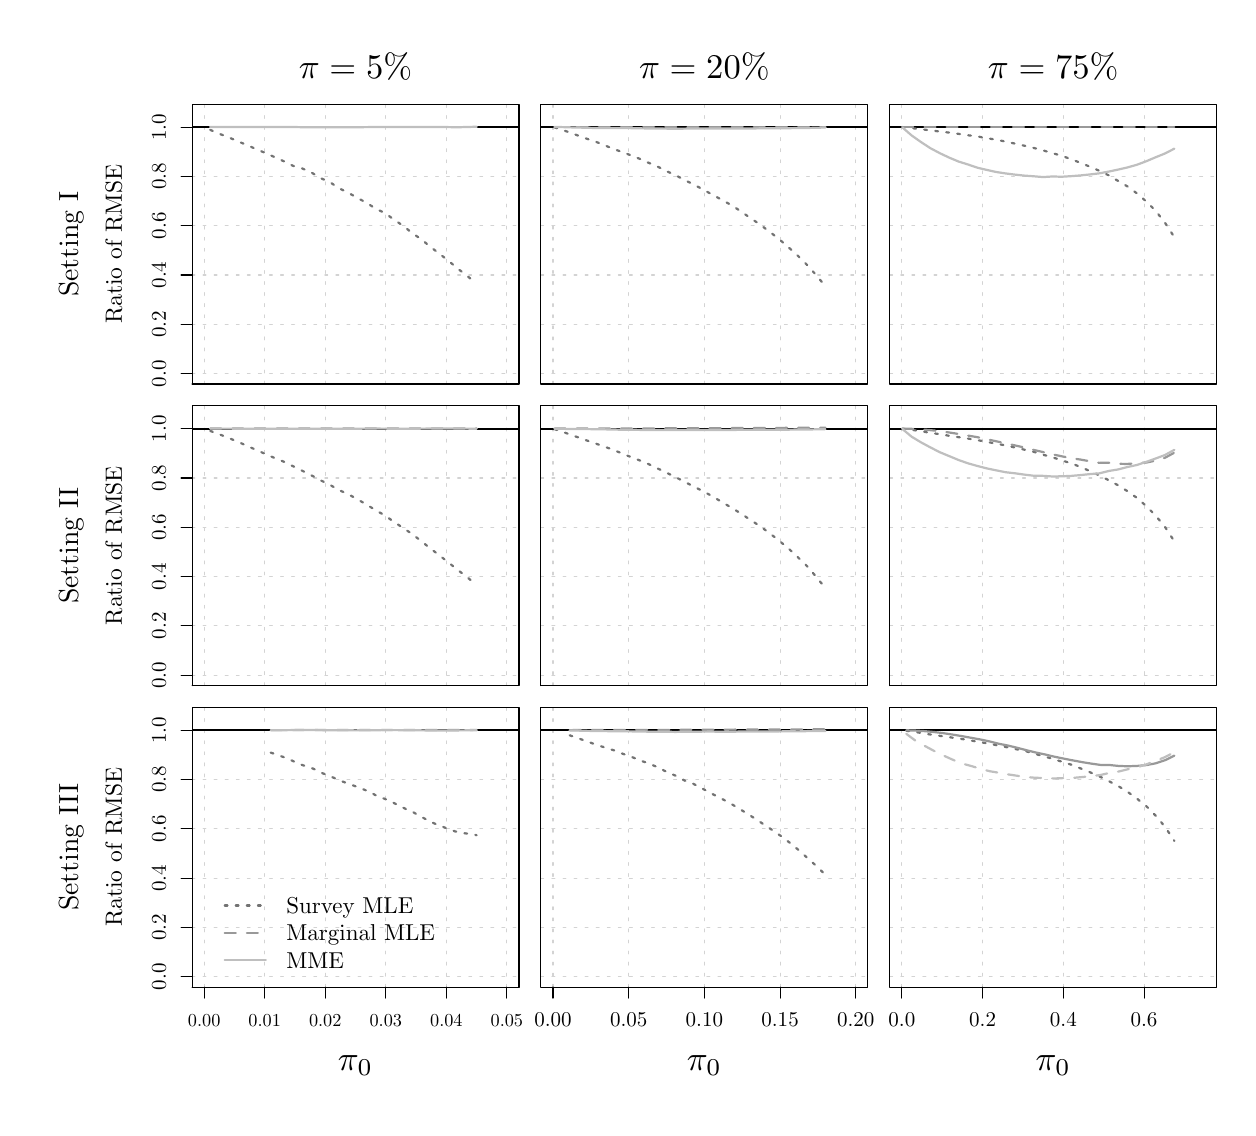
\begin{tikzpicture}[x=1pt,y=1pt]
\definecolor{fillColor}{RGB}{255,255,255}
\path[use as bounding box,fill=fillColor,fill opacity=0.00] (0,0) rectangle (433.62,390.26);
\begin{scope}
\path[clip] ( 55.44,257.53) rectangle (181.50,366.50);
\definecolor{drawColor}{RGB}{0,0,0}

\node[text=drawColor,anchor=base,inner sep=0pt, outer sep=0pt, scale=  0.66] at (118.47,231.40) {Simulation ID};

\node[text=drawColor,rotate= 90.00,anchor=base,inner sep=0pt, outer sep=0pt, scale=  0.66] at ( 34.06,312.01) {Ratio of RMSE};
\end{scope}
\begin{scope}
\path[clip] (  0.00,  0.00) rectangle (433.62,390.26);
\definecolor{drawColor}{RGB}{0,0,0}

\path[draw=drawColor,line width= 0.4pt,line join=round,line cap=round] ( 59.40,265.23) -- ( 59.40,354.34);

\path[draw=drawColor,line width= 0.4pt,line join=round,line cap=round] ( 59.40,265.23) -- ( 55.44,265.23);

\path[draw=drawColor,line width= 0.4pt,line join=round,line cap=round] ( 59.40,283.06) -- ( 55.44,283.06);

\path[draw=drawColor,line width= 0.4pt,line join=round,line cap=round] ( 59.40,300.88) -- ( 55.44,300.88);

\path[draw=drawColor,line width= 0.4pt,line join=round,line cap=round] ( 59.40,318.70) -- ( 55.44,318.70);

\path[draw=drawColor,line width= 0.4pt,line join=round,line cap=round] ( 59.40,336.52) -- ( 55.44,336.52);

\path[draw=drawColor,line width= 0.4pt,line join=round,line cap=round] ( 59.40,354.34) -- ( 55.44,354.34);

\node[text=drawColor,rotate= 90.00,anchor=base,inner sep=0pt, outer sep=0pt, scale=  0.76] at ( 49.90,265.23) {0.0};

\node[text=drawColor,rotate= 90.00,anchor=base,inner sep=0pt, outer sep=0pt, scale=  0.76] at ( 49.90,283.06) {0.2};

\node[text=drawColor,rotate= 90.00,anchor=base,inner sep=0pt, outer sep=0pt, scale=  0.76] at ( 49.90,300.88) {0.4};

\node[text=drawColor,rotate= 90.00,anchor=base,inner sep=0pt, outer sep=0pt, scale=  0.76] at ( 49.90,318.70) {0.6};

\node[text=drawColor,rotate= 90.00,anchor=base,inner sep=0pt, outer sep=0pt, scale=  0.76] at ( 49.90,336.52) {0.8};

\node[text=drawColor,rotate= 90.00,anchor=base,inner sep=0pt, outer sep=0pt, scale=  0.76] at ( 49.90,354.34) {1.0};
\end{scope}
\begin{scope}
\path[clip] ( 59.40,261.49) rectangle (177.54,362.54);
\definecolor{drawColor}{RGB}{211,211,211}

\path[draw=drawColor,line width= 0.4pt,dash pattern=on 1pt off 3pt ,line join=round,line cap=round] ( 63.78,261.49) -- ( 63.78,362.54);

\path[draw=drawColor,line width= 0.4pt,dash pattern=on 1pt off 3pt ,line join=round,line cap=round] ( 85.65,261.49) -- ( 85.65,362.54);

\path[draw=drawColor,line width= 0.4pt,dash pattern=on 1pt off 3pt ,line join=round,line cap=round] (107.53,261.49) -- (107.53,362.54);

\path[draw=drawColor,line width= 0.4pt,dash pattern=on 1pt off 3pt ,line join=round,line cap=round] (129.41,261.49) -- (129.41,362.54);

\path[draw=drawColor,line width= 0.4pt,dash pattern=on 1pt off 3pt ,line join=round,line cap=round] (151.29,261.49) -- (151.29,362.54);

\path[draw=drawColor,line width= 0.4pt,dash pattern=on 1pt off 3pt ,line join=round,line cap=round] (173.16,261.49) -- (173.16,362.54);

\path[draw=drawColor,line width= 0.4pt,dash pattern=on 1pt off 3pt ,line join=round,line cap=round] ( 59.40,265.23) -- (177.54,265.23);

\path[draw=drawColor,line width= 0.4pt,dash pattern=on 1pt off 3pt ,line join=round,line cap=round] ( 59.40,283.06) -- (177.54,283.06);

\path[draw=drawColor,line width= 0.4pt,dash pattern=on 1pt off 3pt ,line join=round,line cap=round] ( 59.40,300.88) -- (177.54,300.88);

\path[draw=drawColor,line width= 0.4pt,dash pattern=on 1pt off 3pt ,line join=round,line cap=round] ( 59.40,318.70) -- (177.54,318.70);

\path[draw=drawColor,line width= 0.4pt,dash pattern=on 1pt off 3pt ,line join=round,line cap=round] ( 59.40,336.52) -- (177.54,336.52);

\path[draw=drawColor,line width= 0.4pt,dash pattern=on 1pt off 3pt ,line join=round,line cap=round] ( 59.40,354.34) -- (177.54,354.34);
\end{scope}
\begin{scope}
\path[clip] (  0.00,  0.00) rectangle (433.62,390.26);
\definecolor{drawColor}{RGB}{0,0,0}

\path[draw=drawColor,line width= 0.4pt,line join=round,line cap=round] ( 59.40,261.49) --
	(177.54,261.49) --
	(177.54,362.54) --
	( 59.40,362.54) --
	( 59.40,261.49);
\end{scope}
\begin{scope}
\path[clip] ( 59.40,261.49) rectangle (177.54,362.54);
\definecolor{drawColor}{RGB}{0,0,0}

\path[draw=drawColor,line width= 0.8pt,line join=round,line cap=round] ( 59.40,354.34) -- (177.54,354.34);
\definecolor{drawColor}{gray}{0.45}

\path[draw=drawColor,line width= 0.8pt,dash pattern=on 1pt off 3pt ,line join=round,line cap=round] ( 65.96,353.33) --
	( 69.28,351.91) --
	( 72.60,350.62) --
	( 75.92,349.23) --
	( 79.24,347.82) --
	( 82.56,346.39) --
	( 85.88,344.97) --
	( 89.20,343.50) --
	( 92.52,342.00) --
	( 95.84,340.34) --
	( 99.16,339.40) --
	(102.48,337.95) --
	(105.80,335.90) --
	(109.12,334.51) --
	(112.43,332.24) --
	(115.75,330.68) --
	(119.07,328.75) --
	(122.39,327.03) --
	(125.71,324.86) --
	(129.03,323.30) --
	(132.35,320.92) --
	(135.67,318.66) --
	(138.99,316.00) --
	(142.31,313.73) --
	(145.63,310.99) --
	(148.95,308.45) --
	(152.27,305.83) --
	(155.59,303.05) --
	(158.91,300.45) --
	(162.23,297.78);
\definecolor{drawColor}{gray}{0.60}

\path[draw=drawColor,line width= 0.8pt,dash pattern=on 4pt off 4pt ,line join=round,line cap=round] ( 65.96,354.34) --
	( 69.28,354.34) --
	( 72.60,354.34) --
	( 75.92,354.34) --
	( 79.24,354.34) --
	( 82.56,354.34) --
	( 85.88,354.34) --
	( 89.20,354.34) --
	( 92.52,354.34) --
	( 95.84,354.34) --
	( 99.16,354.34) --
	(102.48,354.34) --
	(105.80,354.34) --
	(109.12,354.34) --
	(112.43,354.34) --
	(115.75,354.34) --
	(119.07,354.34) --
	(122.39,354.34) --
	(125.71,354.34) --
	(129.03,354.34) --
	(132.35,354.34) --
	(135.67,354.34) --
	(138.99,354.34) --
	(142.31,354.34) --
	(145.63,354.34) --
	(148.95,354.34) --
	(152.27,354.34) --
	(155.59,354.34) --
	(158.91,354.34) --
	(162.23,354.34);
\definecolor{drawColor}{gray}{0.75}

\path[draw=drawColor,line width= 0.8pt,line join=round,line cap=round] ( 65.96,354.34) --
	( 69.28,354.34) --
	( 72.60,354.34) --
	( 75.92,354.36) --
	( 79.24,354.36) --
	( 82.56,354.36) --
	( 85.88,354.34) --
	( 89.20,354.33) --
	( 92.52,354.33) --
	( 95.84,354.35) --
	( 99.16,354.30) --
	(102.48,354.29) --
	(105.80,354.29) --
	(109.12,354.26) --
	(112.43,354.27) --
	(115.75,354.26) --
	(119.07,354.29) --
	(122.39,354.32) --
	(125.71,354.35) --
	(129.03,354.36) --
	(132.35,354.37) --
	(135.67,354.36) --
	(138.99,354.34) --
	(142.31,354.35) --
	(145.63,354.40) --
	(148.95,354.39) --
	(152.27,354.32) --
	(155.59,354.28) --
	(158.91,354.37) --
	(162.23,354.45);
\end{scope}
\begin{scope}
\path[clip] (  0.00,  0.00) rectangle (433.62,390.26);
\definecolor{drawColor}{RGB}{0,0,0}

\node[text=drawColor,rotate= 90.00,anchor=base,inner sep=0pt, outer sep=0pt, scale=  1.00] at ( 18.22,312.01) {Setting I};

\node[text=drawColor,rotate= 90.00,anchor=base,inner sep=0pt, outer sep=0pt, scale=  0.85] at ( 34.06,312.01) {Ratio of RMSE};

\node[text=drawColor,anchor=base,inner sep=0pt, outer sep=0pt, scale=  1.25] at (118.47,372.04) {$\pi = 5\%$};
\end{scope}
\begin{scope}
\path[clip] (181.50,257.53) rectangle (307.56,366.50);
\definecolor{drawColor}{RGB}{0,0,0}

\node[text=drawColor,anchor=base,inner sep=0pt, outer sep=0pt, scale=  0.66] at (244.53,231.40) {Simulation ID};

\node[text=drawColor,rotate= 90.00,anchor=base,inner sep=0pt, outer sep=0pt, scale=  0.66] at (160.12,312.01) {Ratio of RMSE};
\end{scope}
\begin{scope}
\path[clip] (185.46,261.49) rectangle (303.60,362.54);
\definecolor{drawColor}{RGB}{211,211,211}

\path[draw=drawColor,line width= 0.4pt,dash pattern=on 1pt off 3pt ,line join=round,line cap=round] (189.84,261.49) -- (189.84,362.54);

\path[draw=drawColor,line width= 0.4pt,dash pattern=on 1pt off 3pt ,line join=round,line cap=round] (217.18,261.49) -- (217.18,362.54);

\path[draw=drawColor,line width= 0.4pt,dash pattern=on 1pt off 3pt ,line join=round,line cap=round] (244.53,261.49) -- (244.53,362.54);

\path[draw=drawColor,line width= 0.4pt,dash pattern=on 1pt off 3pt ,line join=round,line cap=round] (271.88,261.49) -- (271.88,362.54);

\path[draw=drawColor,line width= 0.4pt,dash pattern=on 1pt off 3pt ,line join=round,line cap=round] (299.22,261.49) -- (299.22,362.54);

\path[draw=drawColor,line width= 0.4pt,dash pattern=on 1pt off 3pt ,line join=round,line cap=round] (185.46,265.23) -- (303.60,265.23);

\path[draw=drawColor,line width= 0.4pt,dash pattern=on 1pt off 3pt ,line join=round,line cap=round] (185.46,283.06) -- (303.60,283.06);

\path[draw=drawColor,line width= 0.4pt,dash pattern=on 1pt off 3pt ,line join=round,line cap=round] (185.46,300.88) -- (303.60,300.88);

\path[draw=drawColor,line width= 0.4pt,dash pattern=on 1pt off 3pt ,line join=round,line cap=round] (185.46,318.70) -- (303.60,318.70);

\path[draw=drawColor,line width= 0.4pt,dash pattern=on 1pt off 3pt ,line join=round,line cap=round] (185.46,336.52) -- (303.60,336.52);

\path[draw=drawColor,line width= 0.4pt,dash pattern=on 1pt off 3pt ,line join=round,line cap=round] (185.46,354.34) -- (303.60,354.34);
\end{scope}
\begin{scope}
\path[clip] (  0.00,  0.00) rectangle (433.62,390.26);
\definecolor{drawColor}{RGB}{0,0,0}

\path[draw=drawColor,line width= 0.4pt,line join=round,line cap=round] (185.46,261.49) --
	(303.60,261.49) --
	(303.60,362.54) --
	(185.46,362.54) --
	(185.46,261.49);
\end{scope}
\begin{scope}
\path[clip] (185.46,261.49) rectangle (303.60,362.54);
\definecolor{drawColor}{RGB}{0,0,0}

\path[draw=drawColor,line width= 0.8pt,line join=round,line cap=round] (185.46,354.34) -- (303.60,354.34);
\definecolor{drawColor}{gray}{0.45}

\path[draw=drawColor,line width= 0.8pt,dash pattern=on 1pt off 3pt ,line join=round,line cap=round] (190.38,354.23) --
	(193.76,353.10) --
	(197.13,351.94) --
	(200.51,350.64) --
	(203.89,349.51) --
	(207.26,348.30) --
	(210.64,346.85) --
	(214.01,345.59) --
	(217.39,344.35) --
	(220.77,343.03) --
	(224.14,341.53) --
	(227.52,340.11) --
	(230.89,338.39) --
	(234.27,336.86) --
	(237.65,335.08) --
	(241.02,333.41) --
	(244.40,331.57) --
	(247.77,329.73) --
	(251.15,327.85) --
	(254.53,326.01) --
	(257.90,323.73) --
	(261.28,321.39) --
	(264.65,319.12) --
	(268.03,316.56) --
	(271.41,313.96) --
	(274.78,311.01) --
	(278.16,307.99) --
	(281.53,304.60) --
	(284.91,300.89) --
	(288.29,296.74);
\definecolor{drawColor}{gray}{0.60}

\path[draw=drawColor,line width= 0.8pt,dash pattern=on 4pt off 4pt ,line join=round,line cap=round] (190.38,354.34) --
	(193.76,354.34) --
	(197.13,354.34) --
	(200.51,354.34) --
	(203.89,354.34) --
	(207.26,354.34) --
	(210.64,354.34) --
	(214.01,354.34) --
	(217.39,354.34) --
	(220.77,354.34) --
	(224.14,354.34) --
	(227.52,354.34) --
	(230.89,354.34) --
	(234.27,354.34) --
	(237.65,354.34) --
	(241.02,354.34) --
	(244.40,354.34) --
	(247.77,354.34) --
	(251.15,354.34) --
	(254.53,354.34) --
	(257.90,354.34) --
	(261.28,354.34) --
	(264.65,354.34) --
	(268.03,354.34) --
	(271.41,354.34) --
	(274.78,354.34) --
	(278.16,354.34) --
	(281.53,354.34) --
	(284.91,354.34) --
	(288.29,354.34);
\definecolor{drawColor}{gray}{0.75}

\path[draw=drawColor,line width= 0.8pt,line join=round,line cap=round] (190.38,354.38) --
	(193.76,354.31) --
	(197.13,354.20) --
	(200.51,354.12) --
	(203.89,354.04) --
	(207.26,354.02) --
	(210.64,354.02) --
	(214.01,354.00) --
	(217.39,353.96) --
	(220.77,353.89) --
	(224.14,353.84) --
	(227.52,353.81) --
	(230.89,353.77) --
	(234.27,353.73) --
	(237.65,353.78) --
	(241.02,353.82) --
	(244.40,353.83) --
	(247.77,353.80) --
	(251.15,353.80) --
	(254.53,353.80) --
	(257.90,353.81) --
	(261.28,353.83) --
	(264.65,353.88) --
	(268.03,353.90) --
	(271.41,353.91) --
	(274.78,353.93) --
	(278.16,353.99) --
	(281.53,354.01) --
	(284.91,354.09) --
	(288.29,354.17);
\end{scope}
\begin{scope}
\path[clip] (  0.00,  0.00) rectangle (433.62,390.26);
\definecolor{drawColor}{RGB}{0,0,0}

\node[text=drawColor,anchor=base,inner sep=0pt, outer sep=0pt, scale=  1.25] at (244.53,372.04) {$\pi = 20\%$};
\end{scope}
\begin{scope}
\path[clip] (307.56,257.53) rectangle (433.62,366.50);
\definecolor{drawColor}{RGB}{0,0,0}

\node[text=drawColor,anchor=base,inner sep=0pt, outer sep=0pt, scale=  0.66] at (370.59,231.40) {Simulation ID};

\node[text=drawColor,rotate= 90.00,anchor=base,inner sep=0pt, outer sep=0pt, scale=  0.66] at (286.18,312.01) {Ratio of RMSE};
\end{scope}
\begin{scope}
\path[clip] (311.52,261.49) rectangle (429.66,362.54);
\definecolor{drawColor}{RGB}{211,211,211}

\path[draw=drawColor,line width= 0.4pt,dash pattern=on 1pt off 3pt ,line join=round,line cap=round] (315.90,261.49) -- (315.90,362.54);

\path[draw=drawColor,line width= 0.4pt,dash pattern=on 1pt off 3pt ,line join=round,line cap=round] (345.07,261.49) -- (345.07,362.54);

\path[draw=drawColor,line width= 0.4pt,dash pattern=on 1pt off 3pt ,line join=round,line cap=round] (374.24,261.49) -- (374.24,362.54);

\path[draw=drawColor,line width= 0.4pt,dash pattern=on 1pt off 3pt ,line join=round,line cap=round] (403.41,261.49) -- (403.41,362.54);

\path[draw=drawColor,line width= 0.4pt,dash pattern=on 1pt off 3pt ,line join=round,line cap=round] (311.52,265.23) -- (429.66,265.23);

\path[draw=drawColor,line width= 0.4pt,dash pattern=on 1pt off 3pt ,line join=round,line cap=round] (311.52,283.06) -- (429.66,283.06);

\path[draw=drawColor,line width= 0.4pt,dash pattern=on 1pt off 3pt ,line join=round,line cap=round] (311.52,300.88) -- (429.66,300.88);

\path[draw=drawColor,line width= 0.4pt,dash pattern=on 1pt off 3pt ,line join=round,line cap=round] (311.52,318.70) -- (429.66,318.70);

\path[draw=drawColor,line width= 0.4pt,dash pattern=on 1pt off 3pt ,line join=round,line cap=round] (311.52,336.52) -- (429.66,336.52);

\path[draw=drawColor,line width= 0.4pt,dash pattern=on 1pt off 3pt ,line join=round,line cap=round] (311.52,354.34) -- (429.66,354.34);
\end{scope}
\begin{scope}
\path[clip] (  0.00,  0.00) rectangle (433.62,390.26);
\definecolor{drawColor}{RGB}{0,0,0}

\path[draw=drawColor,line width= 0.4pt,line join=round,line cap=round] (311.52,261.49) --
	(429.66,261.49) --
	(429.66,362.54) --
	(311.52,362.54) --
	(311.52,261.49);
\end{scope}
\begin{scope}
\path[clip] (311.52,261.49) rectangle (429.66,362.54);
\definecolor{drawColor}{RGB}{0,0,0}

\path[draw=drawColor,line width= 0.8pt,line join=round,line cap=round] (311.52,354.34) -- (429.66,354.34);
\definecolor{drawColor}{gray}{0.45}

\path[draw=drawColor,line width= 0.8pt,dash pattern=on 1pt off 3pt ,line join=round,line cap=round] (316.04,354.34) --
	(319.43,353.96) --
	(322.82,353.56) --
	(326.21,353.16) --
	(329.60,352.72) --
	(332.99,352.34) --
	(336.38,351.88) --
	(339.77,351.38) --
	(343.16,350.95) --
	(346.55,350.35) --
	(349.94,349.77) --
	(353.33,349.11) --
	(356.72,348.36) --
	(360.11,347.61) --
	(363.50,346.81) --
	(366.89,345.91) --
	(370.28,344.92) --
	(373.67,343.95) --
	(377.06,342.72) --
	(380.45,341.41) --
	(383.84,340.02) --
	(387.23,338.54) --
	(390.62,336.90) --
	(394.01,334.88) --
	(397.40,332.89) --
	(400.79,330.39) --
	(404.18,327.48) --
	(407.57,324.10) --
	(410.96,319.77) --
	(414.35,314.54);
\definecolor{drawColor}{gray}{0.60}

\path[draw=drawColor,line width= 0.8pt,dash pattern=on 4pt off 4pt ,line join=round,line cap=round] (316.04,354.34) --
	(319.43,354.34) --
	(322.82,354.34) --
	(326.21,354.34) --
	(329.60,354.34) --
	(332.99,354.34) --
	(336.38,354.34) --
	(339.77,354.34) --
	(343.16,354.34) --
	(346.55,354.34) --
	(349.94,354.34) --
	(353.33,354.34) --
	(356.72,354.34) --
	(360.11,354.34) --
	(363.50,354.34) --
	(366.89,354.34) --
	(370.28,354.34) --
	(373.67,354.34) --
	(377.06,354.34) --
	(380.45,354.34) --
	(383.84,354.34) --
	(387.23,354.34) --
	(390.62,354.34) --
	(394.01,354.34) --
	(397.40,354.34) --
	(400.79,354.34) --
	(404.18,354.34) --
	(407.57,354.34) --
	(410.96,354.34) --
	(414.35,354.34);
\definecolor{drawColor}{gray}{0.75}

\path[draw=drawColor,line width= 0.8pt,line join=round,line cap=round] (316.04,354.24) --
	(319.43,351.30) --
	(322.82,348.91) --
	(326.21,346.70) --
	(329.60,344.90) --
	(332.99,343.30) --
	(336.38,341.88) --
	(339.77,340.82) --
	(343.16,339.66) --
	(346.55,338.86) --
	(349.94,338.11) --
	(353.33,337.59) --
	(356.72,337.16) --
	(360.11,336.80) --
	(363.50,336.56) --
	(366.89,336.27) --
	(370.28,336.48) --
	(373.67,336.39) --
	(377.06,336.60) --
	(380.45,336.87) --
	(383.84,337.22) --
	(387.23,337.62) --
	(390.62,338.25) --
	(394.01,338.97) --
	(397.40,339.75) --
	(400.79,340.71) --
	(404.18,341.98) --
	(407.57,343.42) --
	(410.96,344.79) --
	(414.35,346.54);
\end{scope}
\begin{scope}
\path[clip] (  0.00,  0.00) rectangle (433.62,390.26);
\definecolor{drawColor}{RGB}{0,0,0}

\node[text=drawColor,anchor=base,inner sep=0pt, outer sep=0pt, scale=  1.25] at (370.59,372.04) {$\pi = 75\%$};
\end{scope}
\begin{scope}
\path[clip] ( 55.44,148.57) rectangle (181.50,257.53);
\definecolor{drawColor}{RGB}{0,0,0}

\node[text=drawColor,anchor=base,inner sep=0pt, outer sep=0pt, scale=  0.66] at (118.47,122.43) {Simulation ID};

\node[text=drawColor,rotate= 90.00,anchor=base,inner sep=0pt, outer sep=0pt, scale=  0.66] at ( 34.06,203.05) {Ratio of RMSE};
\end{scope}
\begin{scope}
\path[clip] (  0.00,  0.00) rectangle (433.62,390.26);
\definecolor{drawColor}{RGB}{0,0,0}

\path[draw=drawColor,line width= 0.4pt,line join=round,line cap=round] ( 59.40,156.27) -- ( 59.40,245.37);

\path[draw=drawColor,line width= 0.4pt,line join=round,line cap=round] ( 59.40,156.27) -- ( 55.44,156.27);

\path[draw=drawColor,line width= 0.4pt,line join=round,line cap=round] ( 59.40,174.09) -- ( 55.44,174.09);

\path[draw=drawColor,line width= 0.4pt,line join=round,line cap=round] ( 59.40,191.91) -- ( 55.44,191.91);

\path[draw=drawColor,line width= 0.4pt,line join=round,line cap=round] ( 59.40,209.73) -- ( 55.44,209.73);

\path[draw=drawColor,line width= 0.4pt,line join=round,line cap=round] ( 59.40,227.55) -- ( 55.44,227.55);

\path[draw=drawColor,line width= 0.4pt,line join=round,line cap=round] ( 59.40,245.37) -- ( 55.44,245.37);

\node[text=drawColor,rotate= 90.00,anchor=base,inner sep=0pt, outer sep=0pt, scale=  0.76] at ( 49.90,156.27) {0.0};

\node[text=drawColor,rotate= 90.00,anchor=base,inner sep=0pt, outer sep=0pt, scale=  0.76] at ( 49.90,174.09) {0.2};

\node[text=drawColor,rotate= 90.00,anchor=base,inner sep=0pt, outer sep=0pt, scale=  0.76] at ( 49.90,191.91) {0.4};

\node[text=drawColor,rotate= 90.00,anchor=base,inner sep=0pt, outer sep=0pt, scale=  0.76] at ( 49.90,209.73) {0.6};

\node[text=drawColor,rotate= 90.00,anchor=base,inner sep=0pt, outer sep=0pt, scale=  0.76] at ( 49.90,227.55) {0.8};

\node[text=drawColor,rotate= 90.00,anchor=base,inner sep=0pt, outer sep=0pt, scale=  0.76] at ( 49.90,245.37) {1.0};
\end{scope}
\begin{scope}
\path[clip] ( 59.40,152.53) rectangle (177.54,253.57);
\definecolor{drawColor}{RGB}{211,211,211}

\path[draw=drawColor,line width= 0.4pt,dash pattern=on 1pt off 3pt ,line join=round,line cap=round] ( 63.78,152.53) -- ( 63.78,253.57);

\path[draw=drawColor,line width= 0.4pt,dash pattern=on 1pt off 3pt ,line join=round,line cap=round] ( 85.65,152.53) -- ( 85.65,253.57);

\path[draw=drawColor,line width= 0.4pt,dash pattern=on 1pt off 3pt ,line join=round,line cap=round] (107.53,152.53) -- (107.53,253.57);

\path[draw=drawColor,line width= 0.4pt,dash pattern=on 1pt off 3pt ,line join=round,line cap=round] (129.41,152.53) -- (129.41,253.57);

\path[draw=drawColor,line width= 0.4pt,dash pattern=on 1pt off 3pt ,line join=round,line cap=round] (151.29,152.53) -- (151.29,253.57);

\path[draw=drawColor,line width= 0.4pt,dash pattern=on 1pt off 3pt ,line join=round,line cap=round] (173.16,152.53) -- (173.16,253.57);

\path[draw=drawColor,line width= 0.4pt,dash pattern=on 1pt off 3pt ,line join=round,line cap=round] ( 59.40,156.27) -- (177.54,156.27);

\path[draw=drawColor,line width= 0.4pt,dash pattern=on 1pt off 3pt ,line join=round,line cap=round] ( 59.40,174.09) -- (177.54,174.09);

\path[draw=drawColor,line width= 0.4pt,dash pattern=on 1pt off 3pt ,line join=round,line cap=round] ( 59.40,191.91) -- (177.54,191.91);

\path[draw=drawColor,line width= 0.4pt,dash pattern=on 1pt off 3pt ,line join=round,line cap=round] ( 59.40,209.73) -- (177.54,209.73);

\path[draw=drawColor,line width= 0.4pt,dash pattern=on 1pt off 3pt ,line join=round,line cap=round] ( 59.40,227.55) -- (177.54,227.55);

\path[draw=drawColor,line width= 0.4pt,dash pattern=on 1pt off 3pt ,line join=round,line cap=round] ( 59.40,245.37) -- (177.54,245.37);
\end{scope}
\begin{scope}
\path[clip] (  0.00,  0.00) rectangle (433.62,390.26);
\definecolor{drawColor}{RGB}{0,0,0}

\path[draw=drawColor,line width= 0.4pt,line join=round,line cap=round] ( 59.40,152.53) --
	(177.54,152.53) --
	(177.54,253.57) --
	( 59.40,253.57) --
	( 59.40,152.53);
\end{scope}
\begin{scope}
\path[clip] ( 59.40,152.53) rectangle (177.54,253.57);
\definecolor{drawColor}{RGB}{0,0,0}

\path[draw=drawColor,line width= 0.8pt,line join=round,line cap=round] ( 59.40,245.37) -- (177.54,245.37);
\definecolor{drawColor}{gray}{0.45}

\path[draw=drawColor,line width= 0.8pt,dash pattern=on 1pt off 3pt ,line join=round,line cap=round] ( 65.96,244.54) --
	( 69.28,243.32) --
	( 72.60,241.99) --
	( 75.92,240.65) --
	( 79.24,239.14) --
	( 82.56,237.69) --
	( 85.88,236.22) --
	( 89.20,234.77) --
	( 92.52,233.44) --
	( 95.84,231.82) --
	( 99.16,230.18) --
	(102.48,228.52) --
	(105.80,226.71) --
	(109.12,225.12) --
	(112.43,223.19) --
	(115.75,221.72) --
	(119.07,219.89) --
	(122.39,217.96) --
	(125.71,215.91) --
	(129.03,214.03) --
	(132.35,211.68) --
	(135.67,209.47) --
	(138.99,207.27) --
	(142.31,204.63) --
	(145.63,201.99) --
	(148.95,199.45) --
	(152.27,196.82) --
	(155.59,194.17) --
	(158.91,191.60) --
	(162.23,188.86);
\definecolor{drawColor}{gray}{0.60}

\path[draw=drawColor,line width= 0.8pt,dash pattern=on 4pt off 4pt ,line join=round,line cap=round] ( 65.96,245.38) --
	( 69.28,245.38) --
	( 72.60,245.38) --
	( 75.92,245.38) --
	( 79.24,245.39) --
	( 82.56,245.39) --
	( 85.88,245.39) --
	( 89.20,245.40) --
	( 92.52,245.40) --
	( 95.84,245.40) --
	( 99.16,245.40) --
	(102.48,245.41) --
	(105.80,245.41) --
	(109.12,245.41) --
	(112.43,245.41) --
	(115.75,245.42) --
	(119.07,245.42) --
	(122.39,245.42) --
	(125.71,245.42) --
	(129.03,245.43) --
	(132.35,245.43) --
	(135.67,245.44) --
	(138.99,245.43) --
	(142.31,245.44) --
	(145.63,245.44) --
	(148.95,245.44) --
	(152.27,245.45) --
	(155.59,245.45) --
	(158.91,245.45) --
	(162.23,245.46);
\definecolor{drawColor}{gray}{0.75}

\path[draw=drawColor,line width= 0.8pt,line join=round,line cap=round] ( 65.96,245.39) --
	( 69.28,245.38) --
	( 72.60,245.37) --
	( 75.92,245.36) --
	( 79.24,245.36) --
	( 82.56,245.36) --
	( 85.88,245.36) --
	( 89.20,245.35) --
	( 92.52,245.33) --
	( 95.84,245.33) --
	( 99.16,245.35) --
	(102.48,245.35) --
	(105.80,245.34) --
	(109.12,245.31) --
	(112.43,245.32) --
	(115.75,245.32) --
	(119.07,245.35) --
	(122.39,245.38) --
	(125.71,245.39) --
	(129.03,245.37) --
	(132.35,245.35) --
	(135.67,245.34) --
	(138.99,245.34) --
	(142.31,245.37) --
	(145.63,245.39) --
	(148.95,245.42) --
	(152.27,245.44) --
	(155.59,245.39) --
	(158.91,245.37) --
	(162.23,245.34);
\end{scope}
\begin{scope}
\path[clip] (  0.00,  0.00) rectangle (433.62,390.26);
\definecolor{drawColor}{RGB}{0,0,0}

\node[text=drawColor,rotate= 90.00,anchor=base,inner sep=0pt, outer sep=0pt, scale=  1.00] at ( 18.22,203.05) {Setting II};

\node[text=drawColor,rotate= 90.00,anchor=base,inner sep=0pt, outer sep=0pt, scale=  0.85] at ( 34.06,203.05) {Ratio of RMSE};
\end{scope}
\begin{scope}
\path[clip] (181.50,148.57) rectangle (307.56,257.53);
\definecolor{drawColor}{RGB}{0,0,0}

\node[text=drawColor,anchor=base,inner sep=0pt, outer sep=0pt, scale=  0.66] at (244.53,122.43) {Simulation ID};

\node[text=drawColor,rotate= 90.00,anchor=base,inner sep=0pt, outer sep=0pt, scale=  0.66] at (160.12,203.05) {Ratio of RMSE};
\end{scope}
\begin{scope}
\path[clip] (185.46,152.53) rectangle (303.60,253.57);
\definecolor{drawColor}{RGB}{211,211,211}

\path[draw=drawColor,line width= 0.4pt,dash pattern=on 1pt off 3pt ,line join=round,line cap=round] (189.84,152.53) -- (189.84,253.57);

\path[draw=drawColor,line width= 0.4pt,dash pattern=on 1pt off 3pt ,line join=round,line cap=round] (217.18,152.53) -- (217.18,253.57);

\path[draw=drawColor,line width= 0.4pt,dash pattern=on 1pt off 3pt ,line join=round,line cap=round] (244.53,152.53) -- (244.53,253.57);

\path[draw=drawColor,line width= 0.4pt,dash pattern=on 1pt off 3pt ,line join=round,line cap=round] (271.88,152.53) -- (271.88,253.57);

\path[draw=drawColor,line width= 0.4pt,dash pattern=on 1pt off 3pt ,line join=round,line cap=round] (299.22,152.53) -- (299.22,253.57);

\path[draw=drawColor,line width= 0.4pt,dash pattern=on 1pt off 3pt ,line join=round,line cap=round] (185.46,156.27) -- (303.60,156.27);

\path[draw=drawColor,line width= 0.4pt,dash pattern=on 1pt off 3pt ,line join=round,line cap=round] (185.46,174.09) -- (303.60,174.09);

\path[draw=drawColor,line width= 0.4pt,dash pattern=on 1pt off 3pt ,line join=round,line cap=round] (185.46,191.91) -- (303.60,191.91);

\path[draw=drawColor,line width= 0.4pt,dash pattern=on 1pt off 3pt ,line join=round,line cap=round] (185.46,209.73) -- (303.60,209.73);

\path[draw=drawColor,line width= 0.4pt,dash pattern=on 1pt off 3pt ,line join=round,line cap=round] (185.46,227.55) -- (303.60,227.55);

\path[draw=drawColor,line width= 0.4pt,dash pattern=on 1pt off 3pt ,line join=round,line cap=round] (185.46,245.37) -- (303.60,245.37);
\end{scope}
\begin{scope}
\path[clip] (  0.00,  0.00) rectangle (433.62,390.26);
\definecolor{drawColor}{RGB}{0,0,0}

\path[draw=drawColor,line width= 0.4pt,line join=round,line cap=round] (185.46,152.53) --
	(303.60,152.53) --
	(303.60,253.57) --
	(185.46,253.57) --
	(185.46,152.53);
\end{scope}
\begin{scope}
\path[clip] (185.46,152.53) rectangle (303.60,253.57);
\definecolor{drawColor}{RGB}{0,0,0}

\path[draw=drawColor,line width= 0.8pt,line join=round,line cap=round] (185.46,245.37) -- (303.60,245.37);
\definecolor{drawColor}{gray}{0.45}

\path[draw=drawColor,line width= 0.8pt,dash pattern=on 1pt off 3pt ,line join=round,line cap=round] (190.38,245.18) --
	(193.76,244.04) --
	(197.13,242.85) --
	(200.51,241.63) --
	(203.89,240.46) --
	(207.26,239.27) --
	(210.64,238.06) --
	(214.01,236.72) --
	(217.39,235.34) --
	(220.77,234.04) --
	(224.14,232.66) --
	(227.52,231.03) --
	(230.89,229.41) --
	(234.27,227.78) --
	(237.65,226.01) --
	(241.02,224.27) --
	(244.40,222.60) --
	(247.77,220.69) --
	(251.15,218.67) --
	(254.53,216.68) --
	(257.90,214.57) --
	(261.28,212.32) --
	(264.65,210.12) --
	(268.03,207.64) --
	(271.41,204.98) --
	(274.78,202.18) --
	(278.16,199.04) --
	(281.53,195.77) --
	(284.91,191.87) --
	(288.29,187.68);
\definecolor{drawColor}{gray}{0.60}

\path[draw=drawColor,line width= 0.8pt,dash pattern=on 4pt off 4pt ,line join=round,line cap=round] (190.38,245.38) --
	(193.76,245.39) --
	(197.13,245.40) --
	(200.51,245.41) --
	(203.89,245.41) --
	(207.26,245.43) --
	(210.64,245.43) --
	(214.01,245.44) --
	(217.39,245.45) --
	(220.77,245.45) --
	(224.14,245.46) --
	(227.52,245.47) --
	(230.89,245.48) --
	(234.27,245.49) --
	(237.65,245.50) --
	(241.02,245.51) --
	(244.40,245.53) --
	(247.77,245.54) --
	(251.15,245.56) --
	(254.53,245.57) --
	(257.90,245.59) --
	(261.28,245.60) --
	(264.65,245.61) --
	(268.03,245.61) --
	(271.41,245.63) --
	(274.78,245.66) --
	(278.16,245.66) --
	(281.53,245.67) --
	(284.91,245.72) --
	(288.29,245.73);
\definecolor{drawColor}{gray}{0.75}

\path[draw=drawColor,line width= 0.8pt,line join=round,line cap=round] (190.38,245.35) --
	(193.76,245.28) --
	(197.13,245.24) --
	(200.51,245.22) --
	(203.89,245.18) --
	(207.26,245.14) --
	(210.64,245.06) --
	(214.01,244.99) --
	(217.39,244.96) --
	(220.77,244.92) --
	(224.14,244.87) --
	(227.52,244.84) --
	(230.89,244.83) --
	(234.27,244.88) --
	(237.65,244.89) --
	(241.02,244.91) --
	(244.40,244.84) --
	(247.77,244.86) --
	(251.15,244.89) --
	(254.53,244.90) --
	(257.90,244.93) --
	(261.28,244.95) --
	(264.65,244.98) --
	(268.03,244.95) --
	(271.41,245.00) --
	(274.78,245.00) --
	(278.16,245.03) --
	(281.53,245.03) --
	(284.91,245.13) --
	(288.29,245.19);
\end{scope}
\begin{scope}
\path[clip] (307.56,148.57) rectangle (433.62,257.53);
\definecolor{drawColor}{RGB}{0,0,0}

\node[text=drawColor,anchor=base,inner sep=0pt, outer sep=0pt, scale=  0.66] at (370.59,122.43) {Simulation ID};

\node[text=drawColor,rotate= 90.00,anchor=base,inner sep=0pt, outer sep=0pt, scale=  0.66] at (286.18,203.05) {Ratio of RMSE};
\end{scope}
\begin{scope}
\path[clip] (311.52,152.53) rectangle (429.66,253.57);
\definecolor{drawColor}{RGB}{211,211,211}

\path[draw=drawColor,line width= 0.4pt,dash pattern=on 1pt off 3pt ,line join=round,line cap=round] (315.90,152.53) -- (315.90,253.57);

\path[draw=drawColor,line width= 0.4pt,dash pattern=on 1pt off 3pt ,line join=round,line cap=round] (345.07,152.53) -- (345.07,253.57);

\path[draw=drawColor,line width= 0.4pt,dash pattern=on 1pt off 3pt ,line join=round,line cap=round] (374.24,152.53) -- (374.24,253.57);

\path[draw=drawColor,line width= 0.4pt,dash pattern=on 1pt off 3pt ,line join=round,line cap=round] (403.41,152.53) -- (403.41,253.57);

\path[draw=drawColor,line width= 0.4pt,dash pattern=on 1pt off 3pt ,line join=round,line cap=round] (311.52,156.27) -- (429.66,156.27);

\path[draw=drawColor,line width= 0.4pt,dash pattern=on 1pt off 3pt ,line join=round,line cap=round] (311.52,174.09) -- (429.66,174.09);

\path[draw=drawColor,line width= 0.4pt,dash pattern=on 1pt off 3pt ,line join=round,line cap=round] (311.52,191.91) -- (429.66,191.91);

\path[draw=drawColor,line width= 0.4pt,dash pattern=on 1pt off 3pt ,line join=round,line cap=round] (311.52,209.73) -- (429.66,209.73);

\path[draw=drawColor,line width= 0.4pt,dash pattern=on 1pt off 3pt ,line join=round,line cap=round] (311.52,227.55) -- (429.66,227.55);

\path[draw=drawColor,line width= 0.4pt,dash pattern=on 1pt off 3pt ,line join=round,line cap=round] (311.52,245.37) -- (429.66,245.37);
\end{scope}
\begin{scope}
\path[clip] (  0.00,  0.00) rectangle (433.62,390.26);
\definecolor{drawColor}{RGB}{0,0,0}

\path[draw=drawColor,line width= 0.4pt,line join=round,line cap=round] (311.52,152.53) --
	(429.66,152.53) --
	(429.66,253.57) --
	(311.52,253.57) --
	(311.52,152.53);
\end{scope}
\begin{scope}
\path[clip] (311.52,152.53) rectangle (429.66,253.57);
\definecolor{drawColor}{RGB}{0,0,0}

\path[draw=drawColor,line width= 0.8pt,line join=round,line cap=round] (311.52,245.37) -- (429.66,245.37);
\definecolor{drawColor}{gray}{0.45}

\path[draw=drawColor,line width= 0.8pt,dash pattern=on 1pt off 3pt ,line join=round,line cap=round] (316.04,245.36) --
	(319.43,244.96) --
	(322.82,244.42) --
	(326.21,243.83) --
	(329.60,243.37) --
	(332.99,242.78) --
	(336.38,242.29) --
	(339.77,241.78) --
	(343.16,241.21) --
	(346.55,240.63) --
	(349.94,239.91) --
	(353.33,239.33) --
	(356.72,238.55) --
	(360.11,237.78) --
	(363.50,236.99) --
	(366.89,235.94) --
	(370.28,235.04) --
	(373.67,233.91) --
	(377.06,232.83) --
	(380.45,231.52) --
	(383.84,230.02) --
	(387.23,228.51) --
	(390.62,226.72) --
	(394.01,224.91) --
	(397.40,222.77) --
	(400.79,220.37) --
	(404.18,217.41) --
	(407.57,213.97) --
	(410.96,209.87) --
	(414.35,204.63);
\definecolor{drawColor}{gray}{0.60}

\path[draw=drawColor,line width= 0.8pt,dash pattern=on 4pt off 4pt ,line join=round,line cap=round] (316.04,245.37) --
	(319.43,245.29) --
	(322.82,245.11) --
	(326.21,244.82) --
	(329.60,244.47) --
	(332.99,243.98) --
	(336.38,243.44) --
	(339.77,242.85) --
	(343.16,242.29) --
	(346.55,241.53) --
	(349.94,240.81) --
	(353.33,240.08) --
	(356.72,239.31) --
	(360.11,238.55) --
	(363.50,237.68) --
	(366.89,236.91) --
	(370.28,236.08) --
	(373.67,235.37) --
	(377.06,234.69) --
	(380.45,234.19) --
	(383.84,233.57) --
	(387.23,233.00) --
	(390.62,233.04) --
	(394.01,232.66) --
	(397.40,232.61) --
	(400.79,232.90) --
	(404.18,233.10) --
	(407.57,233.81) --
	(410.96,234.85) --
	(414.35,236.68);
\definecolor{drawColor}{gray}{0.75}

\path[draw=drawColor,line width= 0.8pt,line join=round,line cap=round] (316.04,245.27) --
	(319.43,242.44) --
	(322.82,240.40) --
	(326.21,238.58) --
	(329.60,236.84) --
	(332.99,235.44) --
	(336.38,234.03) --
	(339.77,232.84) --
	(343.16,231.88) --
	(346.55,231.01) --
	(349.94,230.30) --
	(353.33,229.62) --
	(356.72,229.24) --
	(360.11,228.76) --
	(363.50,228.35) --
	(366.89,228.31) --
	(370.28,228.08) --
	(373.67,228.15) --
	(377.06,228.29) --
	(380.45,228.59) --
	(383.84,228.94) --
	(387.23,229.21) --
	(390.62,230.06) --
	(394.01,230.62) --
	(397.40,231.50) --
	(400.79,232.23) --
	(404.18,233.34) --
	(407.57,234.57) --
	(410.96,235.84) --
	(414.35,237.70);
\end{scope}
\begin{scope}
\path[clip] ( 55.44, 39.60) rectangle (181.50,148.57);
\definecolor{drawColor}{RGB}{0,0,0}

\node[text=drawColor,anchor=base,inner sep=0pt, outer sep=0pt, scale=  0.66] at (118.47, 13.46) {Simulation ID};

\node[text=drawColor,rotate= 90.00,anchor=base,inner sep=0pt, outer sep=0pt, scale=  0.66] at ( 34.06, 94.08) {Ratio of RMSE};
\end{scope}
\begin{scope}
\path[clip] (  0.00,  0.00) rectangle (433.62,390.26);
\definecolor{drawColor}{RGB}{0,0,0}

\path[draw=drawColor,line width= 0.4pt,line join=round,line cap=round] ( 59.40, 47.30) -- ( 59.40,136.41);

\path[draw=drawColor,line width= 0.4pt,line join=round,line cap=round] ( 59.40, 47.30) -- ( 55.44, 47.30);

\path[draw=drawColor,line width= 0.4pt,line join=round,line cap=round] ( 59.40, 65.12) -- ( 55.44, 65.12);

\path[draw=drawColor,line width= 0.4pt,line join=round,line cap=round] ( 59.40, 82.94) -- ( 55.44, 82.94);

\path[draw=drawColor,line width= 0.4pt,line join=round,line cap=round] ( 59.40,100.77) -- ( 55.44,100.77);

\path[draw=drawColor,line width= 0.4pt,line join=round,line cap=round] ( 59.40,118.59) -- ( 55.44,118.59);

\path[draw=drawColor,line width= 0.4pt,line join=round,line cap=round] ( 59.40,136.41) -- ( 55.44,136.41);

\node[text=drawColor,rotate= 90.00,anchor=base,inner sep=0pt, outer sep=0pt, scale=  0.76] at ( 49.90, 47.30) {0.0};

\node[text=drawColor,rotate= 90.00,anchor=base,inner sep=0pt, outer sep=0pt, scale=  0.76] at ( 49.90, 65.12) {0.2};

\node[text=drawColor,rotate= 90.00,anchor=base,inner sep=0pt, outer sep=0pt, scale=  0.76] at ( 49.90, 82.94) {0.4};

\node[text=drawColor,rotate= 90.00,anchor=base,inner sep=0pt, outer sep=0pt, scale=  0.76] at ( 49.90,100.77) {0.6};

\node[text=drawColor,rotate= 90.00,anchor=base,inner sep=0pt, outer sep=0pt, scale=  0.76] at ( 49.90,118.59) {0.8};

\node[text=drawColor,rotate= 90.00,anchor=base,inner sep=0pt, outer sep=0pt, scale=  0.76] at ( 49.90,136.41) {1.0};
\end{scope}
\begin{scope}
\path[clip] ( 59.40, 43.56) rectangle (177.54,144.61);
\definecolor{drawColor}{RGB}{211,211,211}

\path[draw=drawColor,line width= 0.4pt,dash pattern=on 1pt off 3pt ,line join=round,line cap=round] ( 63.78, 43.56) -- ( 63.78,144.61);

\path[draw=drawColor,line width= 0.4pt,dash pattern=on 1pt off 3pt ,line join=round,line cap=round] ( 85.65, 43.56) -- ( 85.65,144.61);

\path[draw=drawColor,line width= 0.4pt,dash pattern=on 1pt off 3pt ,line join=round,line cap=round] (107.53, 43.56) -- (107.53,144.61);

\path[draw=drawColor,line width= 0.4pt,dash pattern=on 1pt off 3pt ,line join=round,line cap=round] (129.41, 43.56) -- (129.41,144.61);

\path[draw=drawColor,line width= 0.4pt,dash pattern=on 1pt off 3pt ,line join=round,line cap=round] (151.29, 43.56) -- (151.29,144.61);

\path[draw=drawColor,line width= 0.4pt,dash pattern=on 1pt off 3pt ,line join=round,line cap=round] (173.16, 43.56) -- (173.16,144.61);

\path[draw=drawColor,line width= 0.4pt,dash pattern=on 1pt off 3pt ,line join=round,line cap=round] ( 59.40, 47.30) -- (177.54, 47.30);

\path[draw=drawColor,line width= 0.4pt,dash pattern=on 1pt off 3pt ,line join=round,line cap=round] ( 59.40, 65.12) -- (177.54, 65.12);

\path[draw=drawColor,line width= 0.4pt,dash pattern=on 1pt off 3pt ,line join=round,line cap=round] ( 59.40, 82.94) -- (177.54, 82.94);

\path[draw=drawColor,line width= 0.4pt,dash pattern=on 1pt off 3pt ,line join=round,line cap=round] ( 59.40,100.77) -- (177.54,100.77);

\path[draw=drawColor,line width= 0.4pt,dash pattern=on 1pt off 3pt ,line join=round,line cap=round] ( 59.40,118.59) -- (177.54,118.59);

\path[draw=drawColor,line width= 0.4pt,dash pattern=on 1pt off 3pt ,line join=round,line cap=round] ( 59.40,136.41) -- (177.54,136.41);
\end{scope}
\begin{scope}
\path[clip] (  0.00,  0.00) rectangle (433.62,390.26);
\definecolor{drawColor}{RGB}{0,0,0}

\path[draw=drawColor,line width= 0.4pt,line join=round,line cap=round] ( 59.40, 43.56) --
	(177.54, 43.56) --
	(177.54,144.61) --
	( 59.40,144.61) --
	( 59.40, 43.56);

\path[draw=drawColor,line width= 0.4pt,line join=round,line cap=round] ( 63.78, 43.56) -- (173.16, 43.56);

\path[draw=drawColor,line width= 0.4pt,line join=round,line cap=round] ( 63.78, 43.56) -- ( 63.78, 39.60);

\path[draw=drawColor,line width= 0.4pt,line join=round,line cap=round] ( 85.65, 43.56) -- ( 85.65, 39.60);

\path[draw=drawColor,line width= 0.4pt,line join=round,line cap=round] (107.53, 43.56) -- (107.53, 39.60);

\path[draw=drawColor,line width= 0.4pt,line join=round,line cap=round] (129.41, 43.56) -- (129.41, 39.60);

\path[draw=drawColor,line width= 0.4pt,line join=round,line cap=round] (151.29, 43.56) -- (151.29, 39.60);

\path[draw=drawColor,line width= 0.4pt,line join=round,line cap=round] (173.16, 43.56) -- (173.16, 39.60);

\node[text=drawColor,anchor=base,inner sep=0pt, outer sep=0pt, scale=  0.66] at ( 63.78, 29.30) {0.00};

\node[text=drawColor,anchor=base,inner sep=0pt, outer sep=0pt, scale=  0.66] at ( 85.65, 29.30) {0.01};

\node[text=drawColor,anchor=base,inner sep=0pt, outer sep=0pt, scale=  0.66] at (107.53, 29.30) {0.02};

\node[text=drawColor,anchor=base,inner sep=0pt, outer sep=0pt, scale=  0.66] at (129.41, 29.30) {0.03};

\node[text=drawColor,anchor=base,inner sep=0pt, outer sep=0pt, scale=  0.66] at (151.29, 29.30) {0.04};

\node[text=drawColor,anchor=base,inner sep=0pt, outer sep=0pt, scale=  0.66] at (173.16, 29.30) {0.05};
\end{scope}
\begin{scope}
\path[clip] ( 59.40, 43.56) rectangle (177.54,144.61);
\definecolor{drawColor}{RGB}{0,0,0}

\path[draw=drawColor,line width= 0.8pt,line join=round,line cap=round] ( 59.40,136.41) -- (177.54,136.41);
\definecolor{drawColor}{gray}{0.45}

\path[draw=drawColor,line width= 0.8pt,dash pattern=on 1pt off 3pt ,line join=round,line cap=round] ( 87.84,128.31) --
	( 90.41,127.40) --
	( 92.97,126.51) --
	( 95.54,125.41) --
	( 98.10,124.22) --
	(100.67,123.31) --
	(103.23,122.49) --
	(105.80,121.15) --
	(108.36,120.13) --
	(110.93,119.07) --
	(113.49,117.97) --
	(116.06,116.99) --
	(118.62,116.08) --
	(121.19,115.08) --
	(123.75,114.02) --
	(126.32,112.55) --
	(128.88,111.66) --
	(131.45,110.53) --
	(134.01,109.27) --
	(136.58,107.96) --
	(139.14,106.88) --
	(141.71,105.35) --
	(144.27,104.04) --
	(146.84,102.75) --
	(149.40,101.74) --
	(151.97,100.71) --
	(154.53, 99.81) --
	(157.10, 99.24) --
	(159.66, 98.95) --
	(162.23, 98.47);
\definecolor{drawColor}{gray}{0.60}

\path[draw=drawColor,line width= 0.8pt,dash pattern=on 4pt off 4pt ,line join=round,line cap=round] ( 87.84,136.43) --
	( 90.41,136.43) --
	( 92.97,136.43) --
	( 95.54,136.43) --
	( 98.10,136.44) --
	(100.67,136.44) --
	(103.23,136.44) --
	(105.80,136.44) --
	(108.36,136.45) --
	(110.93,136.45) --
	(113.49,136.45) --
	(116.06,136.45) --
	(118.62,136.45) --
	(121.19,136.46) --
	(123.75,136.46) --
	(126.32,136.46) --
	(128.88,136.46) --
	(131.45,136.46) --
	(134.01,136.47) --
	(136.58,136.47) --
	(139.14,136.47) --
	(141.71,136.48) --
	(144.27,136.48) --
	(146.84,136.48) --
	(149.40,136.48) --
	(151.97,136.48) --
	(154.53,136.48) --
	(157.10,136.49) --
	(159.66,136.50) --
	(162.23,136.52);
\definecolor{drawColor}{gray}{0.75}

\path[draw=drawColor,line width= 0.8pt,line join=round,line cap=round] ( 87.84,136.38) --
	( 90.41,136.40) --
	( 92.97,136.41) --
	( 95.54,136.44) --
	( 98.10,136.47) --
	(100.67,136.46) --
	(103.23,136.44) --
	(105.80,136.43) --
	(108.36,136.40) --
	(110.93,136.38) --
	(113.49,136.36) --
	(116.06,136.35) --
	(118.62,136.34) --
	(121.19,136.36) --
	(123.75,136.38) --
	(126.32,136.41) --
	(128.88,136.43) --
	(131.45,136.43) --
	(134.01,136.42) --
	(136.58,136.41) --
	(139.14,136.37) --
	(141.71,136.35) --
	(144.27,136.32) --
	(146.84,136.31) --
	(149.40,136.30) --
	(151.97,136.32) --
	(154.53,136.32) --
	(157.10,136.34) --
	(159.66,136.35) --
	(162.23,136.36);
\end{scope}
\begin{scope}
\path[clip] (  0.00,  0.00) rectangle (433.62,390.26);
\definecolor{drawColor}{RGB}{0,0,0}

\node[text=drawColor,rotate= 90.00,anchor=base,inner sep=0pt, outer sep=0pt, scale=  1.00] at ( 18.22, 94.08) {Setting III};

\node[text=drawColor,rotate= 90.00,anchor=base,inner sep=0pt, outer sep=0pt, scale=  0.85] at ( 34.06, 94.08) {Ratio of RMSE};

\node[text=drawColor,anchor=base,inner sep=0pt, outer sep=0pt, scale=  1.25] at (118.47, 13.46) {$\pi_0$};
\end{scope}
\begin{scope}
\path[clip] ( 59.40, 43.56) rectangle (177.54,144.61);
\definecolor{drawColor}{gray}{0.45}

\path[draw=drawColor,line width= 0.8pt,dash pattern=on 1pt off 3pt ,line join=round,line cap=round] ( 71.20, 73.04) -- ( 86.05, 73.04);
\definecolor{drawColor}{gray}{0.60}

\path[draw=drawColor,line width= 0.8pt,dash pattern=on 4pt off 4pt ,line join=round,line cap=round] ( 71.20, 63.14) -- ( 86.05, 63.14);
\definecolor{drawColor}{gray}{0.75}

\path[draw=drawColor,line width= 0.8pt,line join=round,line cap=round] ( 71.20, 53.24) -- ( 86.05, 53.24);
\definecolor{drawColor}{RGB}{0,0,0}

\node[text=drawColor,anchor=base west,inner sep=0pt, outer sep=0pt, scale=  0.83] at ( 93.48, 70.20) {Survey MLE};

\node[text=drawColor,anchor=base west,inner sep=0pt, outer sep=0pt, scale=  0.83] at ( 93.48, 60.30) {Marginal MLE};

\node[text=drawColor,anchor=base west,inner sep=0pt, outer sep=0pt, scale=  0.83] at ( 93.48, 50.40) {MME};
\end{scope}
\begin{scope}
\path[clip] (181.50, 39.60) rectangle (307.56,148.57);
\definecolor{drawColor}{RGB}{0,0,0}

\node[text=drawColor,anchor=base,inner sep=0pt, outer sep=0pt, scale=  0.66] at (244.53, 13.46) {Simulation ID};

\node[text=drawColor,rotate= 90.00,anchor=base,inner sep=0pt, outer sep=0pt, scale=  0.66] at (160.12, 94.08) {Ratio of RMSE};
\end{scope}
\begin{scope}
\path[clip] (185.46, 43.56) rectangle (303.60,144.61);
\definecolor{drawColor}{RGB}{211,211,211}

\path[draw=drawColor,line width= 0.4pt,dash pattern=on 1pt off 3pt ,line join=round,line cap=round] (189.84, 43.56) -- (189.84,144.61);

\path[draw=drawColor,line width= 0.4pt,dash pattern=on 1pt off 3pt ,line join=round,line cap=round] (217.18, 43.56) -- (217.18,144.61);

\path[draw=drawColor,line width= 0.4pt,dash pattern=on 1pt off 3pt ,line join=round,line cap=round] (244.53, 43.56) -- (244.53,144.61);

\path[draw=drawColor,line width= 0.4pt,dash pattern=on 1pt off 3pt ,line join=round,line cap=round] (271.88, 43.56) -- (271.88,144.61);

\path[draw=drawColor,line width= 0.4pt,dash pattern=on 1pt off 3pt ,line join=round,line cap=round] (299.22, 43.56) -- (299.22,144.61);

\path[draw=drawColor,line width= 0.4pt,dash pattern=on 1pt off 3pt ,line join=round,line cap=round] (185.46, 47.30) -- (303.60, 47.30);

\path[draw=drawColor,line width= 0.4pt,dash pattern=on 1pt off 3pt ,line join=round,line cap=round] (185.46, 65.12) -- (303.60, 65.12);

\path[draw=drawColor,line width= 0.4pt,dash pattern=on 1pt off 3pt ,line join=round,line cap=round] (185.46, 82.94) -- (303.60, 82.94);

\path[draw=drawColor,line width= 0.4pt,dash pattern=on 1pt off 3pt ,line join=round,line cap=round] (185.46,100.77) -- (303.60,100.77);

\path[draw=drawColor,line width= 0.4pt,dash pattern=on 1pt off 3pt ,line join=round,line cap=round] (185.46,118.59) -- (303.60,118.59);

\path[draw=drawColor,line width= 0.4pt,dash pattern=on 1pt off 3pt ,line join=round,line cap=round] (185.46,136.41) -- (303.60,136.41);
\end{scope}
\begin{scope}
\path[clip] (  0.00,  0.00) rectangle (433.62,390.26);
\definecolor{drawColor}{RGB}{0,0,0}

\path[draw=drawColor,line width= 0.4pt,line join=round,line cap=round] (185.46, 43.56) --
	(303.60, 43.56) --
	(303.60,144.61) --
	(185.46,144.61) --
	(185.46, 43.56);

\path[draw=drawColor,line width= 0.4pt,line join=round,line cap=round] (189.84, 43.56) -- (299.22, 43.56);

\path[draw=drawColor,line width= 0.4pt,line join=round,line cap=round] (189.84, 43.56) -- (189.84, 39.60);

\path[draw=drawColor,line width= 0.4pt,line join=round,line cap=round] (217.18, 43.56) -- (217.18, 39.60);

\path[draw=drawColor,line width= 0.4pt,line join=round,line cap=round] (244.53, 43.56) -- (244.53, 39.60);

\path[draw=drawColor,line width= 0.4pt,line join=round,line cap=round] (271.88, 43.56) -- (271.88, 39.60);

\path[draw=drawColor,line width= 0.4pt,line join=round,line cap=round] (299.22, 43.56) -- (299.22, 39.60);

\node[text=drawColor,anchor=base,inner sep=0pt, outer sep=0pt, scale=  0.76] at (189.84, 29.30) {0.00};

\node[text=drawColor,anchor=base,inner sep=0pt, outer sep=0pt, scale=  0.76] at (217.18, 29.30) {0.05};

\node[text=drawColor,anchor=base,inner sep=0pt, outer sep=0pt, scale=  0.76] at (244.53, 29.30) {0.10};

\node[text=drawColor,anchor=base,inner sep=0pt, outer sep=0pt, scale=  0.76] at (271.88, 29.30) {0.15};

\node[text=drawColor,anchor=base,inner sep=0pt, outer sep=0pt, scale=  0.76] at (299.22, 29.30) {0.20};
\end{scope}
\begin{scope}
\path[clip] (185.46, 43.56) rectangle (303.60,144.61);
\definecolor{drawColor}{RGB}{0,0,0}

\path[draw=drawColor,line width= 0.8pt,line join=round,line cap=round] (185.46,136.41) -- (303.60,136.41);
\definecolor{drawColor}{gray}{0.45}

\path[draw=drawColor,line width= 0.8pt,dash pattern=on 1pt off 3pt ,line join=round,line cap=round] (195.85,134.56) --
	(199.04,133.44) --
	(202.23,132.32) --
	(205.41,131.17) --
	(208.60,130.13) --
	(211.79,129.14) --
	(214.98,127.90) --
	(218.16,126.78) --
	(221.35,125.48) --
	(224.54,124.32) --
	(227.73,122.99) --
	(230.91,121.32) --
	(234.10,119.97) --
	(237.29,118.25) --
	(240.48,117.06) --
	(243.66,115.38) --
	(246.85,113.65) --
	(250.04,111.99) --
	(253.22,110.36) --
	(256.41,108.47) --
	(259.60,106.50) --
	(262.79,104.48) --
	(265.97,102.37) --
	(269.16,100.26) --
	(272.35, 98.05) --
	(275.54, 95.61) --
	(278.72, 92.97) --
	(281.91, 90.09) --
	(285.10, 87.23) --
	(288.29, 84.13);
\definecolor{drawColor}{gray}{0.60}

\path[draw=drawColor,line width= 0.8pt,dash pattern=on 4pt off 4pt ,line join=round,line cap=round] (195.85,136.43) --
	(199.04,136.44) --
	(202.23,136.44) --
	(205.41,136.46) --
	(208.60,136.46) --
	(211.79,136.47) --
	(214.98,136.48) --
	(218.16,136.48) --
	(221.35,136.49) --
	(224.54,136.50) --
	(227.73,136.50) --
	(230.91,136.51) --
	(234.10,136.52) --
	(237.29,136.53) --
	(240.48,136.54) --
	(243.66,136.55) --
	(246.85,136.57) --
	(250.04,136.59) --
	(253.22,136.60) --
	(256.41,136.62) --
	(259.60,136.62) --
	(262.79,136.64) --
	(265.97,136.65) --
	(269.16,136.65) --
	(272.35,136.65) --
	(275.54,136.68) --
	(278.72,136.70) --
	(281.91,136.70) --
	(285.10,136.71) --
	(288.29,136.73);
\definecolor{drawColor}{gray}{0.75}

\path[draw=drawColor,line width= 0.8pt,line join=round,line cap=round] (195.85,136.32) --
	(199.04,136.25) --
	(202.23,136.16) --
	(205.41,136.12) --
	(208.60,136.08) --
	(211.79,136.00) --
	(214.98,136.01) --
	(218.16,135.97) --
	(221.35,135.94) --
	(224.54,135.85) --
	(227.73,135.83) --
	(230.91,135.83) --
	(234.10,135.78) --
	(237.29,135.84) --
	(240.48,135.82) --
	(243.66,135.88) --
	(246.85,135.90) --
	(250.04,135.85) --
	(253.22,135.81) --
	(256.41,135.89) --
	(259.60,135.91) --
	(262.79,135.95) --
	(265.97,135.95) --
	(269.16,135.93) --
	(272.35,135.98) --
	(275.54,136.00) --
	(278.72,135.97) --
	(281.91,136.08) --
	(285.10,136.11) --
	(288.29,136.10);
\end{scope}
\begin{scope}
\path[clip] (  0.00,  0.00) rectangle (433.62,390.26);
\definecolor{drawColor}{RGB}{0,0,0}

\node[text=drawColor,anchor=base,inner sep=0pt, outer sep=0pt, scale=  1.25] at (244.53, 13.46) {$\pi_0$};
\end{scope}
\begin{scope}
\path[clip] (307.56, 39.60) rectangle (433.62,148.57);
\definecolor{drawColor}{RGB}{0,0,0}

\node[text=drawColor,anchor=base,inner sep=0pt, outer sep=0pt, scale=  0.66] at (370.59, 13.46) {Simulation ID};

\node[text=drawColor,rotate= 90.00,anchor=base,inner sep=0pt, outer sep=0pt, scale=  0.66] at (286.18, 94.08) {Ratio of RMSE};
\end{scope}
\begin{scope}
\path[clip] (311.52, 43.56) rectangle (429.66,144.61);
\definecolor{drawColor}{RGB}{211,211,211}

\path[draw=drawColor,line width= 0.4pt,dash pattern=on 1pt off 3pt ,line join=round,line cap=round] (315.90, 43.56) -- (315.90,144.61);

\path[draw=drawColor,line width= 0.4pt,dash pattern=on 1pt off 3pt ,line join=round,line cap=round] (345.07, 43.56) -- (345.07,144.61);

\path[draw=drawColor,line width= 0.4pt,dash pattern=on 1pt off 3pt ,line join=round,line cap=round] (374.24, 43.56) -- (374.24,144.61);

\path[draw=drawColor,line width= 0.4pt,dash pattern=on 1pt off 3pt ,line join=round,line cap=round] (403.41, 43.56) -- (403.41,144.61);

\path[draw=drawColor,line width= 0.4pt,dash pattern=on 1pt off 3pt ,line join=round,line cap=round] (311.52, 47.30) -- (429.66, 47.30);

\path[draw=drawColor,line width= 0.4pt,dash pattern=on 1pt off 3pt ,line join=round,line cap=round] (311.52, 65.12) -- (429.66, 65.12);

\path[draw=drawColor,line width= 0.4pt,dash pattern=on 1pt off 3pt ,line join=round,line cap=round] (311.52, 82.94) -- (429.66, 82.94);

\path[draw=drawColor,line width= 0.4pt,dash pattern=on 1pt off 3pt ,line join=round,line cap=round] (311.52,100.77) -- (429.66,100.77);

\path[draw=drawColor,line width= 0.4pt,dash pattern=on 1pt off 3pt ,line join=round,line cap=round] (311.52,118.59) -- (429.66,118.59);

\path[draw=drawColor,line width= 0.4pt,dash pattern=on 1pt off 3pt ,line join=round,line cap=round] (311.52,136.41) -- (429.66,136.41);
\end{scope}
\begin{scope}
\path[clip] (  0.00,  0.00) rectangle (433.62,390.26);
\definecolor{drawColor}{RGB}{0,0,0}

\path[draw=drawColor,line width= 0.4pt,line join=round,line cap=round] (311.52, 43.56) --
	(429.66, 43.56) --
	(429.66,144.61) --
	(311.52,144.61) --
	(311.52, 43.56);

\path[draw=drawColor,line width= 0.4pt,line join=round,line cap=round] (315.90, 43.56) -- (403.41, 43.56);

\path[draw=drawColor,line width= 0.4pt,line join=round,line cap=round] (315.90, 43.56) -- (315.90, 39.60);

\path[draw=drawColor,line width= 0.4pt,line join=round,line cap=round] (345.07, 43.56) -- (345.07, 39.60);

\path[draw=drawColor,line width= 0.4pt,line join=round,line cap=round] (374.24, 43.56) -- (374.24, 39.60);

\path[draw=drawColor,line width= 0.4pt,line join=round,line cap=round] (403.41, 43.56) -- (403.41, 39.60);

\node[text=drawColor,anchor=base,inner sep=0pt, outer sep=0pt, scale=  0.76] at (315.90, 29.30) {0.0};

\node[text=drawColor,anchor=base,inner sep=0pt, outer sep=0pt, scale=  0.76] at (345.07, 29.30) {0.2};

\node[text=drawColor,anchor=base,inner sep=0pt, outer sep=0pt, scale=  0.76] at (374.24, 29.30) {0.4};

\node[text=drawColor,anchor=base,inner sep=0pt, outer sep=0pt, scale=  0.76] at (403.41, 29.30) {0.6};
\end{scope}
\begin{scope}
\path[clip] (311.52, 43.56) rectangle (429.66,144.61);
\definecolor{drawColor}{RGB}{0,0,0}

\path[draw=drawColor,line width= 0.8pt,line join=round,line cap=round] (311.52,136.41) -- (429.66,136.41);
\definecolor{drawColor}{gray}{0.45}

\path[draw=drawColor,line width= 0.8pt,dash pattern=on 1pt off 3pt ,line join=round,line cap=round] (317.50,136.18) --
	(320.84,135.74) --
	(324.18,135.16) --
	(327.52,134.63) --
	(330.86,134.20) --
	(334.20,133.70) --
	(337.54,133.23) --
	(340.88,132.65) --
	(344.22,132.09) --
	(347.56,131.52) --
	(350.89,130.80) --
	(354.23,130.18) --
	(357.57,129.45) --
	(360.91,128.74) --
	(364.25,127.78) --
	(367.59,126.88) --
	(370.93,125.90) --
	(374.27,124.84) --
	(377.61,123.78) --
	(380.95,122.39) --
	(384.29,121.03) --
	(387.63,119.54) --
	(390.97,117.84) --
	(394.31,116.06) --
	(397.65,113.98) --
	(400.99,111.55) --
	(404.33,108.82) --
	(407.67,105.42) --
	(411.01,101.45) --
	(414.35, 96.40);
\definecolor{drawColor}{gray}{0.60}

\path[draw=drawColor,line width= 0.8pt,line join=round,line cap=round] (317.50,136.38) --
	(320.84,136.26) --
	(324.18,136.05) --
	(327.52,135.74) --
	(330.86,135.33) --
	(334.20,134.82) --
	(337.54,134.27) --
	(340.88,133.66) --
	(344.22,133.06) --
	(347.56,132.35) --
	(350.89,131.50) --
	(354.23,130.86) --
	(357.57,130.04) --
	(360.91,129.17) --
	(364.25,128.35) --
	(367.59,127.64) --
	(370.93,126.84) --
	(374.27,126.16) --
	(377.61,125.50) --
	(380.95,124.88) --
	(384.29,124.33) --
	(387.63,123.86) --
	(390.97,123.82) --
	(394.31,123.47) --
	(397.65,123.37) --
	(400.99,123.50) --
	(404.33,123.80) --
	(407.67,124.45) --
	(411.01,125.56) --
	(414.35,127.20);
\definecolor{drawColor}{gray}{0.75}

\path[draw=drawColor,line width= 0.8pt,dash pattern=on 4pt off 4pt ,line join=round,line cap=round] (317.50,135.08) --
	(320.84,132.59) --
	(324.18,130.71) --
	(327.52,128.91) --
	(330.86,127.27) --
	(334.20,125.76) --
	(337.54,124.38) --
	(340.88,123.48) --
	(344.22,122.48) --
	(347.56,121.59) --
	(350.89,121.03) --
	(354.23,120.44) --
	(357.57,119.93) --
	(360.91,119.47) --
	(364.25,119.20) --
	(367.59,119.13) --
	(370.93,118.96) --
	(374.27,119.09) --
	(377.61,119.15) --
	(380.95,119.46) --
	(384.29,119.79) --
	(387.63,120.21) --
	(390.97,120.98) --
	(394.31,121.48) --
	(397.65,122.32) --
	(400.99,123.04) --
	(404.33,124.09) --
	(407.67,125.36) --
	(411.01,126.69) --
	(414.35,128.46);
\end{scope}
\begin{scope}
\path[clip] (  0.00,  0.00) rectangle (433.62,390.26);
\definecolor{drawColor}{RGB}{0,0,0}

\node[text=drawColor,anchor=base,inner sep=0pt, outer sep=0pt, scale=  1.25] at (370.59, 13.46) {$\pi_0$};
\end{scope}
\end{tikzpicture}
